% Why the order of a saturated chain matters: one component starves the next.
\documentclass[tikz,border=0pt]{standalone}
\usepackage{amsmath}
\usepackage{tikz}
\usetikzlibrary{backgrounds,arrows.meta,positioning}
\definecolor{hdblue}{HTML}{1B4F8A}
\definecolor{hdred}{HTML}{A62B1F}
\definecolor{hdgrey}{HTML}{6B7280}
\begin{document}
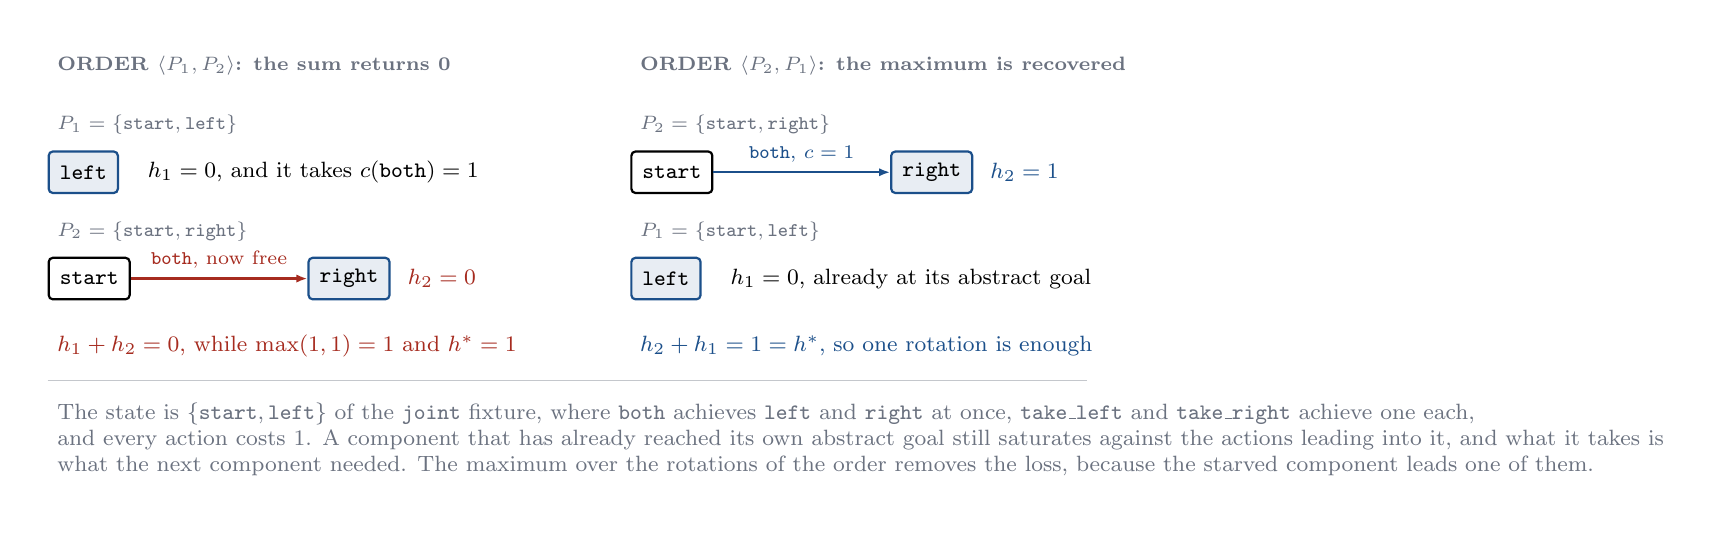
\begin{tikzpicture}[
    show background rectangle, inner frame sep=7pt,
    background rectangle/.style={fill=white},
    font=\footnotesize, >={Latex[length=4pt]},
    st/.style={rectangle,draw=black,thick,fill=white,rounded corners=1.5pt,
               minimum height=15pt,inner xsep=4pt},
    gl/.style={st,draw=hdblue,fill=hdblue!10},
    hdr/.style={font=\scriptsize\bfseries,color=hdgrey}]

  % ---------------- left panel: the order that starves
  \node[hdr,anchor=west] at (0, 2.55) {ORDER $\langle P_1, P_2 \rangle$: the sum returns 0};

  \node[hdr,anchor=west] at (0, 1.80) {$P_1 = \{\texttt{start},\texttt{left}\}$};
  \node[gl,anchor=west] (a1) at (0, 1.20) {\texttt{left}};
  \node[anchor=west] at (1.15, 1.20) {$h_1 = 0$, and it takes $c(\texttt{both}) = 1$};

  \node[hdr,anchor=west] at (0, 0.45) {$P_2 = \{\texttt{start},\texttt{right}\}$};
  \node[st,anchor=west] (a2) at (0,-0.15) {\texttt{start}};
  \node[gl,anchor=west] (b2) at (3.30,-0.15) {\texttt{right}};
  \draw[->,hdred,thick] (a2) -- node[above,font=\scriptsize,hdred,pos=0.5]
        {\texttt{both}, now free} (b2);
  \node[anchor=west,hdred] at (4.45,-0.15) {$h_2 = 0$};

  \node[anchor=west,hdred] at (0,-1.00)
       {$h_1 + h_2 = 0$, while $\max(1,1) = 1$ and $h^{*} = 1$};

  % ---------------- right panel: the rotation that does not
  \begin{scope}[xshift=7.4cm]
  \node[hdr,anchor=west] at (0, 2.55) {ORDER $\langle P_2, P_1 \rangle$: the maximum is recovered};

  \node[hdr,anchor=west] at (0, 1.80) {$P_2 = \{\texttt{start},\texttt{right}\}$};
  \node[st,anchor=west] (a3) at (0, 1.20) {\texttt{start}};
  \node[gl,anchor=west] (b3) at (3.30, 1.20) {\texttt{right}};
  \draw[->,hdblue,thick] (a3) -- node[above,font=\scriptsize,hdblue,pos=0.5]
        {\texttt{both}, $c = 1$} (b3);
  \node[anchor=west,hdblue] at (4.45, 1.20) {$h_2 = 1$};

  \node[hdr,anchor=west] at (0, 0.45) {$P_1 = \{\texttt{start},\texttt{left}\}$};
  \node[gl,anchor=west] (a4) at (0,-0.15) {\texttt{left}};
  \node[anchor=west] at (1.15,-0.15) {$h_1 = 0$, already at its abstract goal};

  \node[anchor=west,hdblue] at (0,-1.00)
       {$h_2 + h_1 = 1 = h^{*}$, so one rotation is enough};
  \end{scope}

  \draw[hdgrey!40] (0,-1.45) -- (13.2,-1.45);
  \node[anchor=north west,align=left,hdgrey] at (0,-1.60)
       {The state is $\{\texttt{start},\texttt{left}\}$ of the \texttt{joint} fixture, where \texttt{both} achieves
        \texttt{left} and \texttt{right} at once, \texttt{take\_left} and \texttt{take\_right} achieve one each,\\
        and every action costs 1. A component that has already reached its own abstract goal still
        saturates against the actions leading into it, and what it takes is\\
        what the next component needed. The maximum over the rotations of the order removes the
        loss, because the starved component leads one of them.};
\end{tikzpicture}
\end{document}
